\section{Architektur}
\label{sec:komponenten:architektur}

Die in dieser Arbeit zugrunde liegende Architektur folgt dem Ansatz von \cite{Truyen2016}, in dem eine containerbasierte
Architektur für \ac{SaaS} Anwendungen vorgestellt wird. Kubernetes spielt hierbei eine wichtige Rolle. Es dient dem State
Managment, der Isolation der Workloads sowie der Authentifizierung für Tenants. Hierbei ist jede Komponente des \ac{SaaS}
mit Kubernetes integriert.

\begin{figure}[h]
  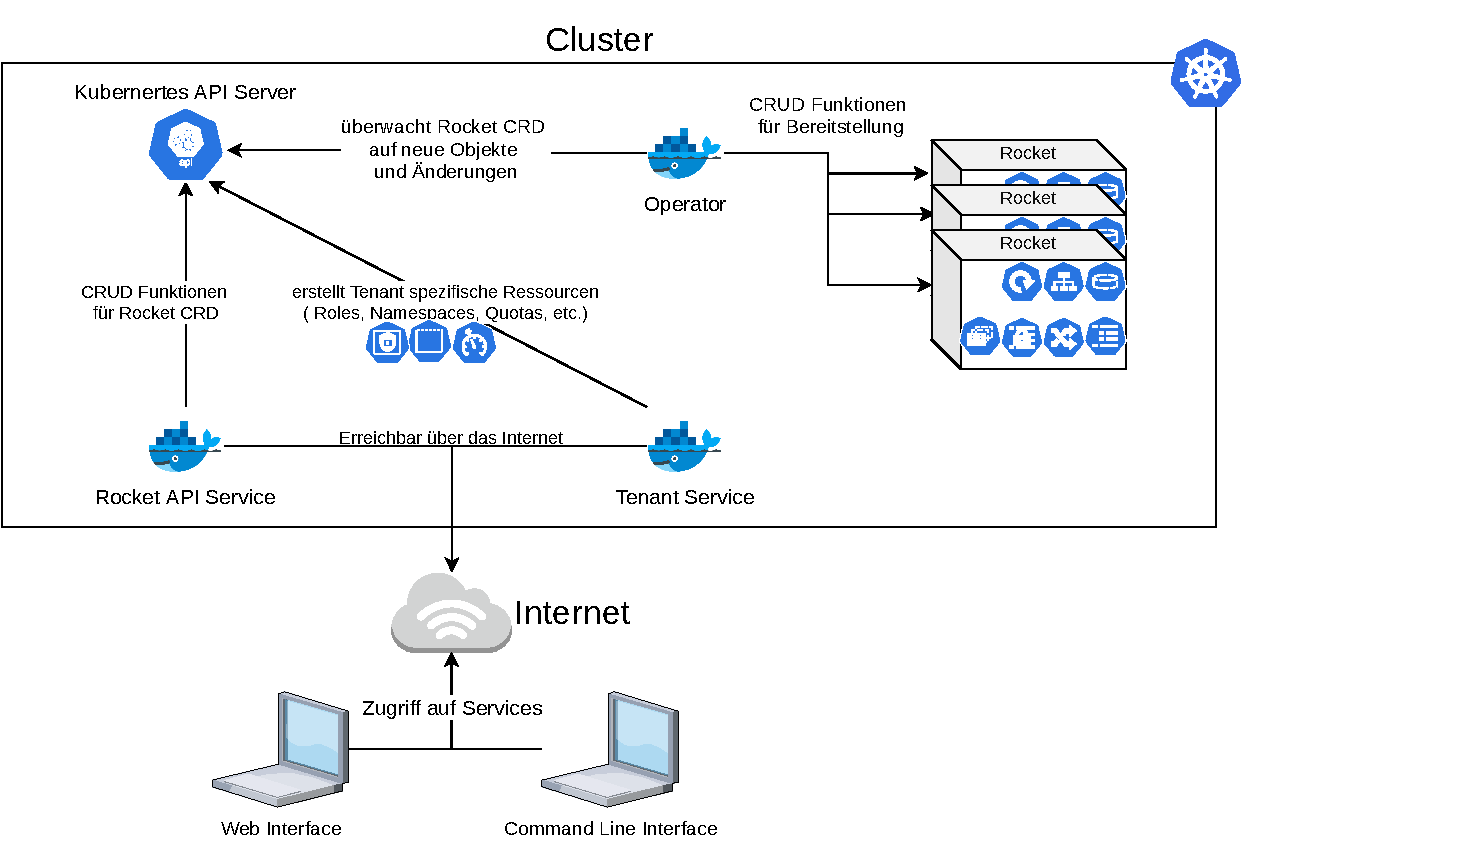
\includegraphics[width=45em]{gfx/chapters/3_komponenten/saas_architecture.pdf}
  \caption{Architektur des \ac{SaaS}}
  \label{fig:architektur}
\end{figure}

In Abbildung \ref{fig:architektur} wird die Architektur der Anwendung beschrieben.
Hierdurch wird deutlich, dass jede Hauptkomponente im Cluster mit der Kubernetes API kommuniziert,
um die gewünschte Konfiguration des Clients zu erzielen.
Jede Komponente des \ac{SaaS} wird ebenfalls als Container im Kubernetes Cluster betrieben.
Diese Konfiguration wird im Cluster mithilfe eines \ac{CR} Objekts, im folgenden Rocket Objekt genannt, dargestellt.
Der Operator dient als Komponente zum tatsächlichen
Erstellen der Rocket.Chat und MongoDB\footnote{Dokumentenorientierte NoSQL-Datenbank \href{https://www.mongodb.com/}{MongoDB}}
Container sowie Netzwerk-, Anwendungs- und Speicherkonfiguration.
Bei einer Änderung der Spezifikation eines Rocket Objekts, wird automatisch eine Synchronisation des 
Clusters vorgenommen, sodass die gewünschte Konfiguration im Cluster deployed ist.

Der Rocket API Service (siehe \ref{sec:komponenten:rocket-api-service}) hat die Aufgabe, 
dass vom Operator definierte \ac{CR} im Kubernetes Cluster zu erstellen,
während der Tenant Service (siehe \ref{sec:komponenten:tenant-service}) für die Konfiguration des Users im Cluster zuständig ist.
Er erstellt Objekte wie beispielsweise Rollen, Namespaces und Quotas für jeden Tenant.

Clients (siehe \ref{sec:komponenten:clients}) haben die Rolle, mit dem Nutzer zu interagieren. 
Als Client kann jegliche Art dienen, zum Beispiel ein \emph{\ac{CLI}} Tool\footnote{Programm zur Interaktion mit dem User via Kommandozeile}
,\emph{\ac{IaC} Tools} oder ein \emph{Web Interface}. Aus Zeitgründen wurde für die Referenzimplementation nur
ein \ac{CLI} Client implementiert.
